\documentclass[10pt]{beamer}

\usetheme{Boadilla}


\usepackage{pgf}
\usepackage[english]{babel}
\usepackage[utf8]{inputenc}

\usepackage{bm}

\usepackage{times}
\usepackage[T1]{fontenc}

%\usepackage{graphicx}
%\usepackage{epstopdf}
%\DeclareGraphicsExtensions{.pdf,.eps,.png,.jpg,.mps} 

\title[\pgfuseimage{department-logo}] %
{Un modelo de Markov para la segmentación automática de señales de audio}

%\subtitle{Include Only If Paper Has a Subtitle}

\author[Rafael de Jesús Robledo Juárez] %
{Rafael de Jesús Robledo Juárez \\
\small{\texttt{rrobledo@cimat.mx}} \\ ~\\
\small{Asesor: Dr. Salvador Ruíz Correa}}


\institute[CIMAT] % (optional, but mostly needed)
{
  Departamento de Ciencias de la Computación\\
  Centro de Investigación en Matemáticas, Guanajuato \\
  ~ \\
  \pgfuseimage{university-logo}
}

\date[Febrero 2013]
{Presentación de Avance de Tesis, 2013}
\subject{Latex Beamer Template}

\pgfdeclareimage[interpolate=true, height=2.5cm]{university-logo}{logos/logo-big}
\pgfdeclareimage[interpolate=true, height=0.5cm]{department-logo}{logos/logo-trans}
%\logo{\pgfuseimage{department-logo}}
\logo{
	\pgfputat{\pgfxy(-0.3, 0)}{
    %\begin{pgfrotateby}{\pgfdegree{30}}
    %  \pgfbox[center,base]{\pgfuseimage{department-logo}}
    %\end{pgfrotateby}
	}
}

% Delete this, if you do not want the table of contents to pop up at
% the beginning of each subsection:

%\AtBeginSubsection[] {
%  \begin{frame}<beamer>{Outline}
%    \tableofcontents[currentsection, currentsubsection]
%  \end{frame}
%}


\usecolortheme[RGB={79, 17, 32}]{structure} 
\setbeamertemplate{navigation symbols}{} 

\begin{document}
\setbeamertemplate{itemize items}[default]
\setbeamertemplate{enumerate items}[default]
\setbeamerfont{section number projected}{series=\bfseries,size={\fontsize{8}{12}}}
\setbeamertemplate{sections/subsections in toc}[square]

\begin{frame}
  \titlepage
\end{frame}

\begin{frame}{Outline}
  \tableofcontents
  % You might wish to add the option [pausesections]
  %\tableofcontents[pausesections]
\end{frame}

\section{Introducción}

\subsection{Motivación}

\begin{frame}{Motivación}
  \begin{itemize}
  	\item
    	La segmentación automática de una señal de audio en zonas homogéneas de acuerdo a las personas que hablan
    se conoce como \textit{speaker diarization}.
    
  	\item
		  Es una etapa importante en el procesamiento de voz. Tanto para reconocimiento como transcripción de voz.
		
  	\item	
  		Es un problema interesante para modelar, pues no se puede considerar que se tiene información a priori.	
  \end{itemize}
\end{frame}

\subsection{Trabajo previo}
\begin{frame}{Trabajo previo}
  You can create overlays\dots
  \begin{itemize}
  \item using the \texttt{pause} command:
    \begin{itemize}
    \item
      First item.
    \item    
      Second item.
    \end{itemize}
  \item
    using overlay specifications:
    \begin{itemize}
    \item
      First item.
    \item
      Second item.
    \end{itemize}
  \item
    using the general \texttt{uncover} command:
    \begin{itemize}
   		\item
        First item.
    	\item
        Second item.
    \end{itemize}
  \end{itemize}
\end{frame}

\section{Procesamiento señal de audio}

\subsection{Preprocesamiento}

\begin{frame}{Elminación de ruido / Detección de silencios}
	\begin{center}
	  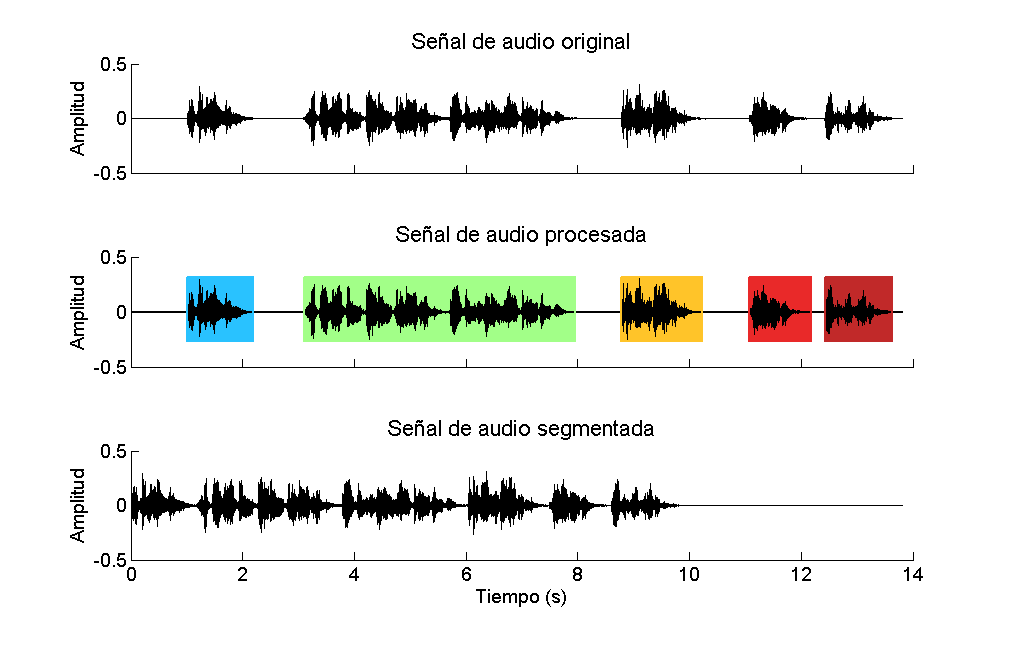
\includegraphics[width=1\textwidth]{gfx/f-silence}
  \end{center}
\end{frame}

\subsection{Obtención de vector de características}

\begin{frame}{Mel Frequency Cepstrum Coefficient}
	\begin{itemize}
		\item \small{FFT (ventana) -> Banco de filtros triangular (Mel Scale) -> Log -> DCT -> MFCC}
	\end{itemize}	
	\begin{center}
	  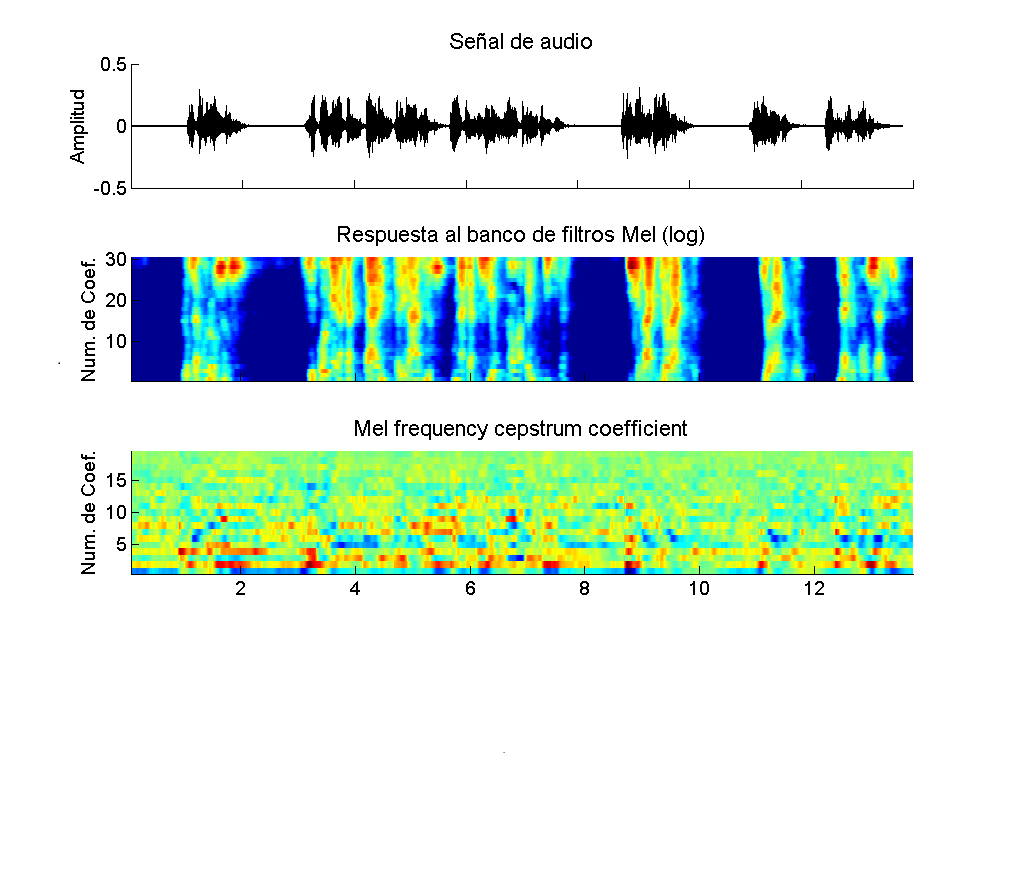
\includegraphics[width=1\textwidth]{gfx/f-mfcc}
  \end{center}
\end{frame}

\section{Modelo}
\subsection{Hidden Markov Model}
\begin{frame}{Hidden Markov Model}
  	\begin{itemize}
   	  \item Cadena de Markov de primer orden
   	  	\begin{center}
	        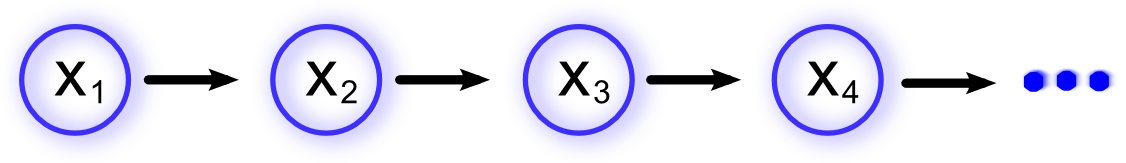
\includegraphics[width=0.4\textwidth]{gfx/mod-mm1}
        \end{center}
        
        \begin{equation}
          \label{eqn:1}
          p(x_1, ..., x_N) 
            ~=~ \prod_{n=1}^N p(x_n ~|~ x_1, ..., x_{n-1}) 
            ~=~ p(x_1) \prod_{n=2}^N p(x_n ~|~ x_{n-1}) 
        \end{equation} 
		  \item Modelo estocástico de Markov en el que el estado de la cadena es parcialmente observado.
		  	\begin{center}
	        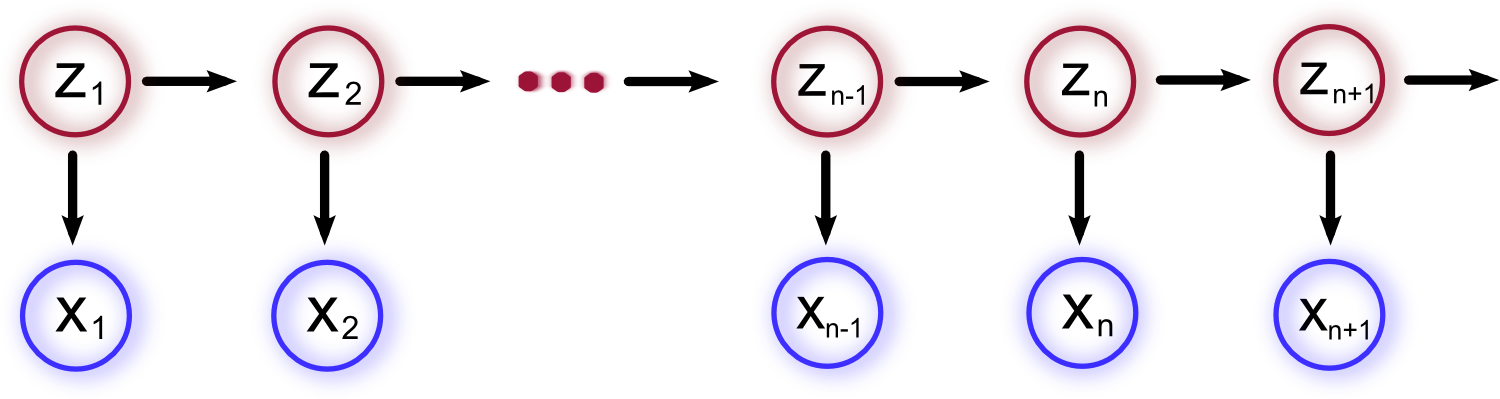
\includegraphics[width=0.5\textwidth]{gfx/mod-hmm}
        \end{center}
		  \item Modelar proceso bivariado en el tiempo. Una variable observada y una variable latente asociada.
	\end{itemize}	
\end{frame}

\begin{frame}{Hidden Markov Model}
  \begin{itemize}
    \item Agregar una variable latente $z_n$ (discreta), que corresponda a cada observación $x_n$.
      \begin{align}
        z_{n+1} &\perp z_{n-1} ~|~ z_{n} \\
        p(x_1, ..., x_N, z_1, ..., z_N) &~=~ p(z_1) \left [ \prod_{n=2}^N p(z_n ~|~ z_{n-1}) \right ] 
          \prod_{n=1}^N p(x_n ~|~ z_{n}).
      \end{align}
      
    \item Mezcla de distribuciones en la que la densidad tiene un distribución dada por $p(x | z)$      
  \end{itemize}
\end{frame}

\begin{frame}{Parámetros del HMM}
  \begin{itemize}
    \item Probabilidad de cambio entre estados dada una \alert{matriz de transición} $\mathbf{A}$
      \begin{align}
        A_{jk} &\equiv p(z_{nk} = 1 ~|~  z_{n-1, j} = 1) \\
        p(z_n ~|~ z_{n-1}, \mathbf{A}) &= \prod_{k=1}^K \prod_{j=1}^K A_{jk}^{z_{{n-1}, j} \cdot z_{n,k}}
      \end{align}      
    \item \alert{Vector de distribución inicial} $\bm{\pi}$ para variable latente.
      \begin{align}
        \pi_k &\equiv p(z_{1k}) \\
        p(z_1 ~|~ \pi) &= \prod_{k=1}^K \pi_k^{z_{1k}}
      \end{align}       
    \item \alert{Probabilidad de emisión} de una variable observada $x_n$ dada una variable latente $z_n$.
      \begin{equation}
        p(x_n ~|~ z_n, \phi) = \prod_{k=1}^K p(x_n ~|~ \phi_k) ^ {z_{nk}}
      \end{equation}
  \end{itemize}
\end{frame}

\subsection{Resolver HMM con EM}

\begin{frame}{HMM con EM}
  \begin{itemize}
    \item Probabilidad conjunta del modelo
      \begin{equation}
        p(\mathbf{X}, \mathbf{Z} ~|~ \theta)        
          = p(z_1 ~|~ \pi) \left[ \prod_{n=2}^N p(z_n ~|~ z_{n-1}, \mathbf{A}) \right]
          \prod_{n=1}^N p(x_n ~|~ z_n, \phi)
      \end{equation}
      
      \item Parámetros del modelo $\theta = \lbrace \bm{\pi}, \mathbf{A}, \phi \rbrace$
      
      \item Función de verosimilitud completa
        \begin{equation}
          \mathcal{Q}(\theta, \theta^{old}) = \sum_{\mathbf{Z}} p(\mathbf{Z} ~|~ \mathbf{X}, \theta^{old})
              \log p(\mathbf{X}, \mathbf{Z} ~|~ \theta)
        \end{equation}
        
      \item Prob. marginal de una variable latente, prob. conjunta de dos variables latentes consecutivas
        \begin{align}
          \gamma(z_n) &= p(z_n ~|~ \mathbf{X}, \theta^{old}) \\
          \xi(z_{n-1}, z_n) &= p(z_{n-1}, z_n ~|~ \mathbf{X}, \theta^{old})
        \end{align}
  \end{itemize}
\end{frame}

\begin{frame}{HMM con EM}
  \begin{itemize}
      \item Prob. marginal de $z_nk = 1$, prob. conjunta de $z_{n-1,j}, z_{nk}$
        \begin{align}
          \gamma(z_{nk}) &= \mathbb{E} \left[ z_{nk} \right] = \sum_Z  \gamma(\mathbf{z}) z_{nk} \label{eq-13} \\
          \xi(z_{n-1,j}, z_{nk}) &= \mathbb{E} \left[z_{n-1, j} \cdot z_{nk} \right] = 
            \sum_Z  \gamma(\mathbf{z}) z_{n-1, j} \cdot z_{nk} \label{eq-14}
        \end{align}  
        
        \item Función de verosimilitud completa (reescrita con \eqref{eq-13}, \eqref{eq-14})
          \begin{equation}
            \begin{split}
              \mathcal{Q}(\theta, \theta^{old}) = 
              \sum_{k=1}^K \gamma(z_{1k}) \log \pi_k + 
              \sum_{n=2}^N \sum_{j=1}^K \sum_{k=1}^K \xi(z_{n-1,j}, z_{nk}) \log A_{jk} + \\
              \sum_{n=1}^N \sum_{k=1}^K \gamma(z_{nk}) \log p(x_n ~|~ \phi_k)
            \end{split}
          \end{equation}
          
         \item Parámetros estimados por EM: 
         \begin{equation}
           \pi_k = \frac{\gamma(z_{1k})}{\sum_{j=1}^K \gamma(z_1j)}, ~~
           A_{jk} = \sum_{n=2}^N \frac{\xi(z_{n-1,j}, z_{nk})}{ \sum_{l=1}^K \xi(z_{n-1,j}, z_{nl})}
         \end{equation}
  \end{itemize}
\end{frame}

\begin{frame}{Algoritmo backward-forward}
  \begin{align}
  \gamma(z_n) &= p(z_n ~|~ X) = \frac{p(X ~|~ z_n) p(z_n)}{p(X)} \\
  \gamma(z_n) &= \frac{p(x_1, ..., x_n, z_n)p(x_{n+1}, ..., x_N ~|~ z_n)}{p(X)} \\
  \gamma(z_n) &= \frac{\alpha(z_n) \beta(z_n)}{p(X)} \\  
  \end{align}
  donde 
  \begin{align}
    \alpha(z_n) &\equiv p(x_1, ..., x_n, z_n) \\
    \beta(z_n) &\equiv p(x_{n+1}, ..., x_N ~|~ z_n)  \\
    \alpha(z_n) &= p(x_n ~|~ z_n) \sum_{z_{n-1}} \alpha(z_n ~|~ z_{n-1}) \\
    \alpha(z_1) &= p(z_1) p(x_1 ~|~ z_1) = \prod_{k=1}^K \lbrace {\pi_k p(x_1 ~|~ \phi_k)} \rbrace ^ {z_{1k}}
  \end{align}  
\end{frame}

\begin{frame}{Algoritmo backward-forward}
  \begin{align}
    \beta(z_n) = \sum_{z_{n+1}} \beta(z_{n+1})p(x_{n+1} ~|~ z_{n+1}) p(z_{n+1} ~|~ z_n)
  \end{align}  
\end{frame}

\subsection{Bootstrap}
\begin{frame}{Bootstrap}
\end{frame}

\section{Pruebas}

\subsection{Pruebas con datos sintéticos}

\begin{frame}{Numero fijo de speakers}
\end{frame}

\begin{frame}{Numero variable de speakers}
\end{frame}

\section*{Resumen}

\begin{frame}{Resumen}
  \begin{itemize}
  \item
    The \alert{first main message} of your talk in one or two lines.
  \item
    The \alert{second main message} of your talk in one or two lines.
  \item
    Perhaps a \alert{third message}, but not more than that.
  \end{itemize}
  
  % The following outlook is optional.
  \vskip0pt plus.5fill
  \begin{itemize}
  \item
    Outlook
    \begin{itemize}
    \item
      Something you haven't solved.
    \item
      Something else you haven't solved.
    \end{itemize}
  \end{itemize}
\end{frame}

\section{Trabajo futuro}

\begin{frame}{Trabajo futuro}
\end{frame}

% All of the following is optional and typically not needed. 
\appendix
\section<presentation>*{\appendixname}
\subsection<presentation>*{Referencias}

\begin{frame}[allowframebreaks]
  \frametitle<presentation>{Referencias}
    
  \begin{thebibliography}{10}
    
  \beamertemplatebookbibitems

  \bibitem{Author1990}
    A.~Author.
    \newblock {\em Handbook of Everything}.
    \newblock Some Press, 1990.
 
    
  \beamertemplatearticlebibitems

  \bibitem{Someone2000}
    S.~Someone.
    \newblock On this and that.
    \newblock {\em Journal of This and That}, 2(1):50--100,
    2000.
  \end{thebibliography}
\end{frame}

\end{document}